%devoir2.tex
%Par Guillaume Lahaie et Guy Francoeur
%LAHG04077707 FRAG21127205
%
%%%%%%%%%%%%%%%%%%%%%%%%%%%%%%%%%%%%%%%%%
% Simple Sectioned Essay Template
% LaTeX Template
%
% This template has been downloaded from:
% http://www.latextemplates.com
%
% Note:
% The \lipsum[#] commands throughout this template generate dummy text
% to fill the template out. These commands should all be removed when 
% writing essay content.
%
%%%%%%%%%%%%%%%%%%%%%%%%%%%%%%%%%%%%%%%%%

%----------------------------------------------------------------------------------------
%	PACKAGES AND OTHER DOCUMENT CONFIGURATIONS
%----------------------------------------------------------------------------------------

\documentclass[12pt,letterpaper]{article} % Default font size is 12pt, it can be changed here
\renewcommand{\familydefault}{\rmdefault}
\renewcommand{\thesubsection}{\alph{subsection}}

%Pour l'encodage avec accents
\usepackage[utf8x]{inputenc}
\usepackage[french,english]{babel}

%\usepackage{helvet}
%\renewcommand{\familydefault}{\sfdefault}

%Pour INF7235 - devoir 2
\usepackage{pdflscape}
\usepackage{multirow}
\usepackage{mathtools}
\usepackage{algorithm2e}

\usepackage{afterpage}
\usepackage{appendix}
\usepackage{graphicx} % Required for including pictures
\usepackage{epstopdf}

\usepackage[left=2.2cm,top=2.2cm,right=2.2cm,bottom=2.2cm,nohead]{geometry} % Required to change the page size to A4
\geometry{letterpaper} % Set the page size to be A4 as opposed to the default US Letter

\usepackage{float} % Allows putting an [H] in \begin{figure} to specify the exact location of the figure
\linespread{1.2} % Line spacing

%\setlength\parindent{0pt} % Uncomment to remove all indentation from paragraphs


%Comportement d'un paragraphe
\setlength{\parskip}{\baselineskip}%
\setlength{\parindent}{0pt}%

%Widows/orphans
\widowpenalty10000
\clubpenalty10000

\usepackage[colorlinks=true]{hyperref}

%Meta-info
\title{INF7235 - devoir 2}
\author{Guillaume Lahaie, Guy Francoeur}
\date{Remise: 23 avril 2014}

\hypersetup{
  pdftitle={INF7235 - devoir 2},
  pdfauthor={Guillaume Lahaie et Guy Francoeur}
  pdfsubject={devoir 2 - MPI Factorisation LU}
  pdfkeywords={MPI C, factorisation LU}
}

\newcommand\blankpage{%
  \null
  \thispagestyle{empty}%
  \addtocounter{page}{-1}%
  \newpage}

\begin{document}
\selectlanguage{french}
\fussy

%----------------------------------------------------------------------------------------
%	TITLE PAGE
%----------------------------------------------------------------------------------------

\begin{titlepage}

\newcommand{\HRule}{\rule{\linewidth}{0.5mm}} % Defines a new command for the horizontal lines, change thickness here

\center % Center everything on the page

\textsc{\LARGE Université du Québec à Montréal}\\[1.5cm] % Name of your university/college
\textsc{\Large INF7235}\\[0.5cm] % Major heading such as course name

\HRule \\[1.5cm]
{ \huge \bfseries Devoir 2}\\[0.4cm] % Title of your document
\HRule \\[1.5cm]

\begin{minipage}{0.4\textwidth}
\begin{flushleft} \large
\emph{Par:}\\
Guillaume Lahaie - LAHG04077707\\
Guy Francoeur -  FRAG21127205
\end{flushleft}
\end{minipage}
~
\begin{minipage}{0.4\textwidth}
\begin{flushright} \large
\emph{Remis à:} \\
Guy Tremblay% Supervisor's Name
\end{flushright}
\end{minipage}\\[4cm]

{\large \emph{Date de remise:} \\ Le 23 avril 2014}\\[3cm] % Date, change the \today to a set date if you want to be precise

%\includegraphics{Logo}\\[1cm] % Include a department/university logo - this will require the graphicx package

\vfill % Fill the rest of the page with whitespace

\end{titlepage}
\blankpage

%----------------------------------------------------------------------------------------
%	TABLE OF CONTENTS
%----------------------------------------------------------------------------------------

\tableofcontents % Include a table of contents

\newpage % Begins the essay on a new page instead of on the same page as the table of contents 

%----------------------------------------------------------------------------------------
% SECTIONS DU DOCUMENT
%----------------------------------------------------------------------------------------


\section{Description du problème}

Nous avons décidé d'étudier la parallélisation de la décomposition LU. Regardons tout d'abord ce qu'est
cette décomposition, quelle est son utilité. Nous regarderons ensuite l'algorithme permettant de
décomposer une matrice.

\subsection{Décomposition LU}

Supposons que nous avons une matrice $A$ carrée, de dimensions $n*n$. Alors, s'il est possible de
réduire la matrice $A$ sous forme échelonnée, il est possible de décomposer $A$ tel que
$A = LU$, où $L$ est une matrice triangulaire inférieure, et $U$ est une matrice triangulaire supérieure\cite{lay2006LinAlgitsAppThiedi}.

Voyons un exemple tiré de \emph{Linear Algebra And Its Applications}.

$A =
\begin{pmatrix}
3 & -7 & -2 & 2 \\
-3 & 5 & 1 & 0 \\
6 & -4 & 0 & -5 \\
-9 & 5 & -5 & 12
\end{pmatrix}$

Cette matrice peut être décomposée en forme LU:

$A =
\begin{pmatrix}
3 & -7 & -2 & 2 \\
-3 & 5 & 1 & 0 \\
6 & -4 & 0 & -5 \\
-9 & 5 & -5 & 12
\end{pmatrix} 
=
\begin{pmatrix}
1 & 0 & 0 & 0 \\
-1 & 1 & 0 & 0 \\
2 & -5 & 1 & 0 \\
-3 & 8 & 3 & 1
\end{pmatrix}
\begin{pmatrix}
3 & -7 & -2 & 2 \\
0 & -2 & -1 & 2 \\
0 & 0 & -1 & 1 \\
0 & 0 & 0 & -1
\end{pmatrix} 
= LU$

La décomposition LU permet de résoudre un système d'équations linéaires, d'inverser une
matrice ou encore de calculer le déterminant de la matrice\cite{wikipedia-LU}.

La résolution d'un système d'équations linéaires effectué par un ordinateur 
est plus efficace par une factorisation LU que par le calcul de la matrice inverse.
En effet, la décomposition permet de calculer le résultat en moins d'opérations
à virgule flottante, et en obtenant un résultat plus précis\cite{lay2006LinAlgitsAppThiedi}.

\subsection{Algorithme de décomposition}

L'algorithme de décomposition s'apparente à l'élimination de Gauss. En effet, comme chaque
étape de l'élimination de Gauss peut être représentée par une matrice élémentaire,
la matrice $L$ est la multiplication de toutes les matrices élémentaires permettant
d'obtenir $U$\cite{lay2006LinAlgitsAppThiedi}.

Il est possible de travailler soit sur les lignes de la matrice $A$, ou encore selon
l'algorithme de Doolittle, colonne par colonne\cite{wikipedia-LU}.

Voici un algorithme séquentiel de factorisation LU proposé par 
Heath pour une matrice de dimensions $n \times n$ \cite{parallel-lu}:

\begin{algorithm}
 \SetKwInput{Fonction}{fonction}
 \SetKwInput{Donnees}{donnees}
 \SetKwInput{Antecedents}{antécédents}
 \SetKwInput{Consequents}{conséquents}
 \Fonction{LU($A$)}
 \Donnees{$A$: une matrice de dimensions $n \times n$}
 \Sortie{$A$: une matrice triangulaire supérieure\\
         $L$: une matrice triangulaire inférieure}
 \Deb{
    \Pour{$k \longleftarrow 1$ à $n-1$}{
      \Pour{$i \longleftarrow k+1$ à $n$}{
	$L_{ik} = \frac{A_{ik}}{A_{kk}}$}
	
      \Pour{$j \longleftarrow k+1$ à $n$}{
	\Pour{$i \longleftarrow k+1$ à $n$}{
	  $A_{ij} = A_{ij} - A_{ik} \times A_{kj}$
	  }
	  }
	  }
}          
\end{algorithm}

Cet algorithme a une complexité temporelle de $O(n^3)$. Pour une très grande matrice, il peut
donc être utile de paralléliser les opérations.

Pour le moment, nous ne traitons pas des permutations des lignes de la matrice. 
Selon Heath, la permutation est nécessaire pour vérifier l'existence d'une solution et
pour assurer la stabilité numérique du résultat\cite{parallel-lu}.

\section{Approche de parallélisation PCAM}

Nous nous basons sur le texte de Heath\cite{parallel-lu} pour appliquer l'approche PCAM de
Foster\cite{foster1994comsysthaintHigPerForForM} à ce problème.

\subsection{Partition}

Selon Heath, nous pouvons utiliser un parallélisme de résultat ici, et appliquer les
étapes de l'algorithme sur chaque valeur de la matrice\cite{parallel-lu}. 
D'ailleurs, il n'est pas nécessaire d'allouer une seconde matrice pour les résultats 
de la décomposition, il est possible de modifier directement 
la matrice $A$, indicé de $0$ à $n-1$ de cette façon:

$\forall i, j, 0\le i, j, \le n-1$\\
$A_{ij} = u_{ij}$ si $i \le j$\\
$A_{ij} = l_{ij}$ si $i > j$

Pour le partitionnement, il est donc possible d'obtenir la granularité la plus fine en attribuant
à chaque valeur de la matrice $LU$ un processeur. Donc, pour la granularité la plus fine, nous 
avons besoin de $n^2$ processeurs. La figure \ref{figure1} montre les communications à effectuer
avec une granularité fine.

\begin{figure}[h]
\centering
 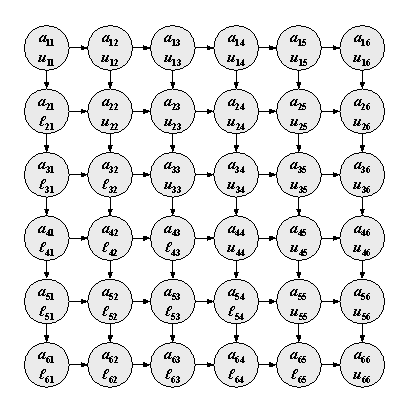
\includegraphics{fine_grain.eps}
 \caption{\label{figure1}Communication pour une granularité très fine. Source: Heath\cite{parallel-lu}}
 
\end{figure}

\newpage
\subsection{Communication}

Heath propose ce modèle de communication pour les tâches à granularité fine\cite{parallel-lu}:
\begin{itemize}
   \item faire une communication de type \emph{broadcast} pour envoyer les valeurs de A à la tâche
    située dans la même colonne, à la ligne suivante
   \item faire une communication de type \emph{broadcast} pour les entrées de L à la tâche
    à la même ligne, mais à la prochaine colonne.
\end{itemize}

Ceci résulterait dans l'algorithme suivant:

\begin{algorithm}
 \SetKwInput{Fonction}{fonction}
 \SetKwInput{Donnees}{donnees}
 \SetKwInput{Antecedents}{antécédents}
 \SetKwInput{Consequents}{conséquents}
 \Deb{
    \Pour{$k \longleftarrow 1$ à $min(i, j)-1$}{
      recevoir broadcast $a_{kj}$ de la tâche $(k, j)$\\
      recevoir broadcast $l_{ik}$ de la tâche $(i, k)$\\
      $a_{ij} = a_{ij} - l_{ik}a_{kj}$
    }
    \Si{$i \le j$} {
      envoyer un broadcast $a_{ij}$ aux tâches $(k, j)$, pour $k = i+1 ... n$
    }
    \Sinon {
      recevoir broadcast $a_{jj}$ de la tâche $(j, j)$\\
      $l_{ij} = a_{ij} / a_{jj}$\\
      envoyer un broadcast $l_{ij}$ aux tâches $(i, k)$, pour $k = j+1 ... n$
    }
}
\caption{Algorithme parallèle à granularité fine de décomposition LU. Source: Heath\cite{parallel-lu}}
\end{algorithm}

\subsection{Agglomération et Mapping}

Selon Health, l'agglomération peut se faire de trois façons, 
exactement comme pour la multiplication de matrices. On peut regrouper les tâches 
par colonnes, par lignes, ou par blocs $k*k$, où $k = \sqrt{p}$, $p$ étant 
le nombre de processeurs disponibles\cite{parallel-lu}.

Comme nous avons déjà vu pour la multiplication de matrices, une agglomération par blocs, ou
une agglomération en deux dimensions, permets de réduire les éléments à communiquer 
à chaque processeur. Toutefois ici, il faut aussi considérer le travail des processeurs. 
En effet, plus nous approchons de la fin du traitement, plus les processeurs traitant 
les premiers blocs, lignes ou colonnes se retrouveront inactifs, ce qui n'est pas optimal.
Heath propose donc une agglomération cyclique pour tenter d'atténuer ce problème.

Andrews propose une approche alternative d'échanges de messages\cite{andrews1999FouMulParDisPro}.
Il serait possible d'utiliser une approche de pipeline circulaire. Un noeud recevrait une
donnée, effectue le calcule nécessaire et ensuite passe l'information au prochain noeud.
Cette méthode nécessite toutefois un très grand nombre de messages, elle pourrait même, selon
Andrews, être moins efficace qu'un méthode séquentielle.

\section{Implémentation à l'aide de MPI}

Nous avons choisi les approches de parallélisation suivante pour la factorisation LU:

\begin{itemize}
 \item agglomération par lignes adjacentes sans pivot partiel
 \item agglomération par lignes adjacentes avec pivot partiel
 \item agglomération par lignes cycliques sans pivot partiel
 \item agglomération par lignes cycliques avec pivot partiel
 \item agglomération par blocs adjacents sans pivot partiel
\end{itemize}

En implémentant deux agglomérations par ligne différentes, nous voulions vérifier le coût
d'avoir des processeurs inactifs sur le temps d'exécution de l'algorithme. Selon Heath, une
agglomération cyclique permet de mieux répartir le travail. 

Nous avons toutefois rencontré
une difficulté à configurer les communications pour ces approches. Lorsqu'un bloc de lignes
a terminé son travail, il n'est plus nécessaire de pour ce bloc de recevoir les messages.
Toutefois, avec des communications globales, il serait alors nécessaire de redéfinir le
communicateur pour enlever ce noeud. Nous avons donc choisi de laisser le noeud dans le
communicateur et pour lui de ne plus faire de travail. Il est toutefois possible de
mettre à jour à chaque communication la taille de la ligne à communiquer. Cela réduit
donc la taille des données à échanger.

Notre seconde approche vise à vérifier la différence entre un regroupement 1D et un regroupement
2D. En théorie, un regroupement 2D est plus efficace, réduisant le nombre de données à 
transférer. Toutefois, cela ajoute un nombre important de communications. Nous voulions donc
vérifier l'impact de l'ajout des communications sur le temps d'exécution. Encore une fois, 
pour l'approche 2D, certaines communications sont superflues, car un bloc peut avoir terminé
ses calculs. Nous n'avons pas ajusté la taille des données à échanger ici, mais chaque bloc 
pourrait calculer ce qu'il doit recevoir ou envoyer à chaque étape de la réduction.

Finalement, nous avons implémenté pour les regroupements 1D des versions avec ou sans
pivot partiel. L'utilisation du pivot partiel est nécessaire pour la factorisation LU
effectuée par logiciels, comme les calculs sont effectués sur des nombres à 
virgule flottante, cela permet de limiter la perte de précision. 
Toutefois, cela nécessite des communications supplémentaires. Nous voulons donc vérifier 
l'effet de ces communications sur l'algorithme. 

Pour implémenter les pivots de lignes dans
les versions 1D,nous avons implémenté deux communications. Premièrement, il faut trouver
la valeur maximum locale dans nos lignes. Ensuite, chaque noeud doit pouvoir déterminer
quel est le maximum global. Nous avons donc utilisé une communication globale de type
\texttt{MPI\_Allgather}. Il serait possible de faire un \texttt{MPI\_Gather} sur le noeud
traitant la ligne actuelle, mais cela nécessiterait ensuite un \texttt{MPI\_Bcast} pour que chaque
noeud sache quel noeud a le maximum. Finalement, il y a une communication point à point
entre le noeud traitant la ligne actuelle et le noeud possédant le maximum global pour
échanger les lignes.

Afin de simplifier le code, nous ne traitons que des matrices carrées ($n\times n$), et
nous nous assurons que $p$, le nombre de noeuds utilisés est un diviseur de $n$ ($n\bmod p = 0$).
De plus, nous ne vérifions pas s'il est vraiment possible de factoriser la matrice en entrée.
Comme nous travaillons sur des matrices de nombres à virgule flottante, une division par 0 
a comme résultat l'infinité, alors que la division $0\div 0$ a comme résultat NaN. Cela ne
cause donc pas une erreur dans l'application.

\section{Tests}

\subsection{Exactitude}
Nous avons tout d'abord vérifié l'exactitude des résultats obtenus par les différents programmes.
Pour ce faire, nous avons pris deux exemples du livre \emph{Linear Algebra And Its Applications}.
Les réponses du livre n'utilisent pas une approche avec pivot partiel. Donc, pour les applications
avec pivot partiel, nous avons utilisé la bibliothèque \emph{scipy} de python pour calculer les résultats.
Ces deux exemples sont des matrices de dimension $4\times 4$, et sont les tests 1 et 2 du 
\texttt{makefile}.

Nous avons ensuite composé à la main un exemple d'une matrice $6 \times 6$, surtout dans le but
de vérifier si, pour l'approche d'agrégation en deux dimensions, notre approche donnait le
bon résultat même si la décomposition n'est pas égale entre les colonnes et les lignes. Il 
s'agit du test 3 du \texttt{makefile}.

Finalement, nous avons généré une matrice de dimensions $30 \times 30$ contenant des
nombres aléatoires de -100 à 100 à l'aide de la bibliothèque \emph{numpy} de python. Nous avons
généré le résultat avec pivot partiel pour avec la méthode lu de scipy, et pour le résultat
sans pivot, nous avons utilisé la version séquentielle (\texttt{lu\_seq.c}). Il est possible
de vérifier le résultat avec le test 4 du \texttt{makefile}.

\subsection{Performance}

Nous avons vérifié la performance en faisant varier la taille du problème, donc de la
matrice en entrée, et aussi en faisant varier le nombre de noeuds traitant la matrice.

Pour la variation de taille de la matrice, nous pris comme cas le plus long un traitement
d'environ cinq minutes, ce qui est une matrice de dimension $9000 \times 9000$, et nous 
avons fait varier par la taille de la matrice par pas de 600. Nous avons utilisé 30 noeuds
pour ces tests.

Nous avons fait varier le nombre de noeuds pour une matrice de dimensions $6000 \times 6000$.
Nous avons fait varier le nombre de noeuds par 5. 

Nous avons effectué chaque test cinq fois sur le cluster turing de l'UQAM. Nous présentons
les temps moyens de ces cinq tests.

\section{Résultats et analyse}

Regardons tout d'abord les temps d'exécution lorsque la taille du problème varie.

\begin{table}[h!]
 \centering
\begin{tabular}{|l|c|c|c|c|c|c|c|}
\hline
\multirow{2}{*}{\bf{Taille}}& \multicolumn{7}{|c|}{\bf{Temps d'exécution}} \\ \cline{2-8}
&\multicolumn{2}{|c|}{Séquentiel} & \multicolumn{2}{|c|}{Lignes adjacentes} &
\multicolumn{2}{|c|}{Lignes cycliques} & Blocs 2D \\ \hline
Pivot: & Non & Oui & Non & Oui & Non & Oui & Non \\ \hline
600 &144.00 &150.00&238.59&1402.43&272.53&1149.44&180.00 \\ \hline
1200&900.00&646.00&686.41&2487.22&800.66&2460.80&481.52 \\ \hline
1800&2554.00&2560.00&1354.99&3986.95&1457.15&4076.69&1596.70 \\ \hline
2400&6298.00&6380.00&2370.27&5877.45&2349.14&6134.99&2790.68 \\ \hline
3000&12564.00&12646.00&3740.311&8466.13&3986.53&9069.08&4451.54 \\ \hline
3600&22516.00&23096.00&5545.11&11514.61&5544.34&11734.38&7473.94 \\ \hline
4200&39104.00&39648.00&7725.77&16702.70&7903.90&15957.55&12985.06 \\ \hline
4800&57214.00&58118.00&12032.52&21961.79&10636.36&20535.12&16321.39\\ \hline
5400&81306.00&81996.00&15268.05&28960.78&14629.14&26050.16&21268.06\\ \hline
6000&116182.00&111878.00&22125.61&36749.59&18930.55&34002.65&32024.31\\ \hline
6600&150456.00&147795.00&28610.95&46104.86&25956.24&42804.06&42667.00\\ \hline
7200&180370.00&164015.00&36316.61&58544.23&32528.77&52619.93&51949.99\\ \hline
7800&210090.00&218315.00&48201.49&71244.06&41082.30&60995.61&70993.46\\ \hline
8400&277252.50&278467.50&63240.01&82108.22&48141.85&72244.99&87997.58\\ \hline
9000&340340.00&341587.50&71683.34&97409.08&57205.19&85498.44&106487.50\\ \hline
\end{tabular}
\caption{\label{1}Temps d'exécution en millisecondes selon la taille de la matrice}
\end{table}


\begin{table}[h!]
 \centering
\begin{tabular}{|l|c|c|c|c|c|}
\hline
\multirow{2}{*}{\bf{Noeuds}}& \multicolumn{5}{|c|}{\bf{Temps d'exécution}} \\ \cline{2-6}
& \multicolumn{2}{|c|}{Lignes adjacentes} & \multicolumn{2}{|c|}{Lignes cycliques} & Blocs 2D \\ \hline
Pivot: & Non & Oui & Non & Oui & Non \\ \hline
5&86643.66&93712.54&61535.74&70586.27&93950.39 \\ \hline
10&56570.81&64257.52&47666.56&54377.69&71341.98 \\ \hline
15&38732.41&48639.95&29941.08&39430.40&54689.67 \\ \hline
20&29766.75&39603.42&26732.55&38319.02&42882.45 \\ \hline
25&24583.56&35341.22&20285.52&34438.64&36690.51 \\ \hline
30&22766.15&37983.02&17947.10&34051.56&30231.72 \\ \hline
\end{tabular}
\caption{Temps d'exécution en millisecondes selon le nombre de noeuds utilisés}
\end{table}
\begin{figure}[h!]
\begin{center}
\includegraphics[angle=-90, width=0.65\linewidth]{noeuds.eps}
\end{center}
\end{figure}
\begin{figure}[h!]
\begin{center}
\includegraphics[angle=-90, width=0.65\linewidth]{noeuds_pivot.eps}
\end{center}
\end{figure}
\begin{figure}[h!]
\begin{center}
\includegraphics[angle=-90, width=0.65\linewidth]{taille.eps}
\end{center}
\end{figure}
\begin{figure}[h!]
\begin{center}
\includegraphics[angle=-90, width=0.65\linewidth]{taille_pivot.eps}
\end{center}
\end{figure}


La table \ref{1} nous permet de faire certains constats. Tout d'abord, lorsque le
problème est de petite taille, le coût des communications est prohibitif, il est
plus efficace d'utiliser la version séquentielle. D'ailleurs, dans ces cas une
approche avec pivot partiel a un temps d'exécution beaucoup plus long que la version
séquentielle. La matrice doit avoir une taille de 2400 ou plus pour obtenir une
accélération positive.

En général, l'utilisation d'une approche de parallélisme par échange de messages
permet de diminuer le temps d'exécution de la factorisation LU. En regardant les
graphes d'accélération, on peut toutefois conclure que pour nos implémentations
de l'algorithme naïf parallèle, avec ou sans pivot, l'accélération n'est pas linéaire.
Si on double le nombre de noeuds, le temps d'exécution ne diminue pas de moitié.

La factorisation LU parallèle par échange de messages nécessite un grand nombre de synchronisations.
Il est impossible d'envoyer les informations nécessaires à un noeud et ensuite d'avoir le résultat
final. Il faut, à chaque traitement de lignes, obtenir les informations nécessaires pour effectuer
la réduction de cette ligne.

L'accélération semble converger autour de 5 ou 6 pour les approches d'agglomération par lignes,
avec l'accélération pour une agglomération cyclique un peu plus élevée. L'accélération est
plus basse pour une approche avec pivot, atteignant des valeurs maximales entre 3 et 4. L'approche
d'agglomération par blocs a une accélération maximale entre 3 et 4, donc notre version est moins
efficace que l'approche 1D. Cela pourrait s'expliquer par notre implémentation inefficace
contenant des échanges de messages superflus.

On peut voir que l'ajout de noeuds permet toutefois d'augmenter l'accélération pour les approches
sans pivot partiel et avec pivot partiel, toutefois le gain en accélération est beaucoup moins
important pour l'approche avec pivot partiel.

\subsection{Agglomération des lignes}
Regardons plus en détail l'effet du choix d'agglomération de lignes. On peut remarquer
que lorsqu'on fait varier la taille du problème, la version à distribution cyclique
est marginalement plus efficace, pour les versions avec et sans pivot. On remarque
que l'écart devient plus important lorsque la taille du problème devient très grande.
Lorsqu'on fait varier le nombre de noeuds traitant le problème, encore une fois l'écart
en efficacité est plus grand lorsque chaque noeud a plus de traitement à faire. On peut
remarquer que lorsqu'on utilise seulement cinq noeuds, les versions à agglomération cyclique
sont plus efficaces que les versions à agglomération adjacente. Ce gain en efficacité
diminue en augmentant le nombre de noeuds.

\subsection{Utilisation du pivot partiel}
Il est difficile de bien analyser l'effet de l'utilisation du pivot partiel sur le
temps d'exécution des programmes, car nous ne savons pas le nombre de pivots
entre noeuds différents, donc le nombre de communications point à point nécessaire.
On peut toutefois remarquer que l'ajout du pivot a un impact sur le temps d'exécution
de la factorisation LU. L'effet semble moins important lorsque le nombre de 
noeuds est bas, ou lorsque la matrice à traiter est très grande. Cela pourrait s'expliquer
par l'augmentation de la chance de trouver le pivot dans son propre noeud plutôt que
dans un autre noeud.

\subsection{Agglomération 1D et 2D}

Notre agglomération en blocs 2D pour la factorisation LU est la moins efficace des trois
que nous avons implémentés sans pivot partiel. Notre approche envoie plus de données que
les deux autres, car nous n'avons pas limité les communications. Il serait possible
d'enlever les communications lorsqu'une ligne ou colonne n'a plus de travail à faire.
Cette approche permettrait de limiter les données transmises, mais il y aurait
toujours plus de synchronisations, qu'une approche à une dimension. Il serait
intéressant de voir l'effet de l'utilisation de communications point à point
pour cette approche.

\section{Conclusion}

La parallélisation de la factorisation LU par échange de messages comporte
plusieurs défis. C'est un algorithme qui demande un nombre élevé de communications
et un grand besoin de synchronisation. De plus, comme on effectue plusieurs
calculs sur des nombres à virgules flottantes, il faut utiliser des méthodes
pour diminuer la perte de précision afin d'obtenir à la fin, un résultat
exact. Il faut aussi s'assurer de bien distribuer les tâches pour éviter
d'avoir des noeuds inactifs, et vérifier s'il est vraiment possible de 
décomposer la matrice.

En utilisant l'approche PCAM de Foster, nous avons utilisé trois approches
d'agglomération des données de la matrice à décomposer: 
par lignes adjacentes, par lignes cycliques et par blocs 2D adjacents. 

Nous avons utilisé des communications collectives pour partager
les informations que chaque noeud a besoin pour effectuer la décomposition.
Cela a comme effet d'effectuer des communications superflues, donc on perd
en performance dans ce cas. Nous croyons que notre agglomération par blocs 2D
est inefficace en partie due à ces problèmes de communication.

Nous avons aussi implémenté le pivot partiel pour les agglomérations par lignes.
Cela augmente le nombre de communications, mais est nécessaire pour obtenir des
résultats précis.

Nos tests démontrent qu'il est possible d'avoir une accélération variant de 3 à
6, selon l'agglomération et l'utilisation du pivot partiel. Cette accélération
semble basse, considérant le nombre de noeuds utilisés.

%%%%%%%%%%%%%%%%%%%%%%%%%%%%%%%%%%%%%%%%%%%%%%%%%%%%%%%%%%%%%%%%%%%%%%%%%%%%%%%
% Bibliographie
%%%%%%%%%%%%%%%%%%%%%%%%%%%%%%%%%%%%%%%%%%%%%%%%%%%%%%%%%%%%%%%%%%%%%%%%%%%%%%%

%Pour le utf8 de bibtex
\begingroup
\inputencoding{latin1}
\bibliographystyle{ieeetr}
\bibliography{devoir2}
\endgroup

\end{document}
